\chapter{Ausgewählte Aspekte}

\section{NGINX sichern mit letsencrypt}

\section{EspWifiManager Implementation}

\section{Die Wichtigkeit von Erase Flash}

\section{ELF vs Bin}

\subsection{ELF}

ELF ist die Abkürzung für Executable and Linkable Format und definiert die Struktur für Binärdateien, Bibliotheken und Core-Dateien. Die formale Spezifikation ermöglicht es dem Betriebssystem, die zugrunde liegenden Maschinenanweisungen korrekt zu interpretieren. ELF-Dateien sind normalerweise die Ausgabe eines Compilers oder Linkers und haben ein Binärformat.
\newline
\newline
Ein häufiges Missverständnis ist, dass ELF-Dateien nur für Binärdateien oder ausführbare Dateien bestimmt sind. Es ist jedoch möglich sie für Teilstücke (Objektcode) verwendet zu können. Ein weiteres Beispiel sind gemeinsam genutzte Bibliotheken oder sogar Core-Dumps (Core- oder a.out-Dateien). Die ELF-Spezifikation wird auch unter Linux für den Kernel selbst und die Linux-Kernelmodule verwendet.


\subsection{Struktur}
Aufgrund des erweiterbaren Designs von ELF-Dateien unterscheidet sich die Struktur je nach Datei. Eine ELF-Datei besteht aus:

\begin{itemize} 
\item ELF-Header
\item Dateidaten
\end{itemize}

Mit dem Befehl readelf können wir uns die Struktur einer Datei ansehen und sie sieht ungefähr so aus:

\begin{figure}[H]
    \begin{center}
        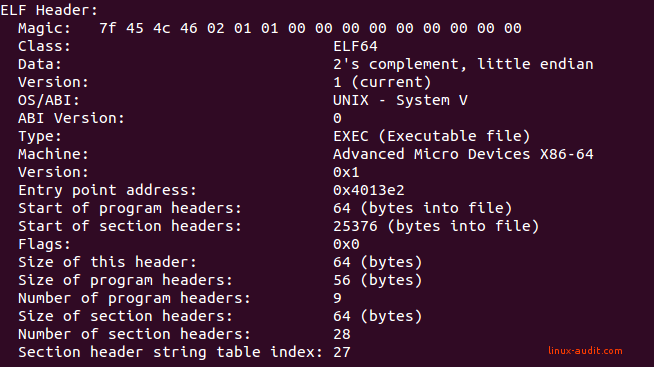
\includegraphics[scale=0.5]{images/elf-header-linux-binary.png}
        \caption{Details einer Elf-binary \cite{details_of_Elf_binary}}
    \end{center}
\end{figure}
 
\subsection{ELF-Header}
Wie in diesem Screenshot zu sehen ist, beginnt der ELF-Header mit etwas Magic. Diese ELF-Header-Magic liefert Informationen über die Datei. Die ersten 4 hexadezimalen Teile definieren, dass dies eine ELF-Datei ist (45 = E, 4c = L, 46 = F), der der Wert 7f vorangestellt ist.
 
Dieser ELF-Header ist obligatorisch. Es stellt sicher, dass Daten während der Verknüpfung oder Ausführung korrekt interpretiert werden. Um die innere Funktionsweise einer ELF-Datei besser zu verstehen, ist es hilfreich zu wissen, dass diese Header-Informationen verwendet werden.
 
\subsubsection{Class}
Nach der ELF-Typdeklaration ist ein Class-feld definiert. Dieser Wert bestimmt die Architektur für die Datei. Es kann sich um eine 32-Bit- (= 01) oder 64-Bit- (= 02) Architektur handeln. Magic zeigt eine 02, die vom Befehl readelf als ELF64-Datei übersetzt wird. Mit anderen Worten, eine ELF-Datei, die die 64-Bit-Architektur verwendet.

\subsubsection{Data}
Der nächste Teil ist das Data-feld. Es kennt zwei Optionen: 01 für LSB (Least Significant Bit), auch als Little-Endian bekannt. Dann gibt es den Wert 02 für MSB (Most Significant Bit, Big-Endian). Dieser spezielle Wert hilft dabei, die verbleibenden Objekte in der Datei korrekt zu interpretieren. Dies ist wichtig, da verschiedene Prozessortypen unterschiedlich mit den eingehenden Anweisungen und Datenstrukturen umgehen. In diesem Fall wird LSB verwendet, was für Prozessoren vom Typ AMD64 üblich ist.

\subsubsection{Version}
Als nächstes folgt eine weitere "01" in der Magic, die die Versionsnummer ist. Derzeit gibt es nur einen Versionstyp: Derzeit ist dies der Wert "01". Also nichts Interessantes zu merken.

\subsubsection{OS / ABI}
Jedes Betriebssystem hat eine große Überlappung in gemeinsamen Funktionen. Darüber hinaus hat jedes von ihnen spezifische oder zumindest geringfügige Unterschiede. Die Definition des richtigen Sets erfolgt über eine Application Binary Interface (ABI). Auf diese Weise wissen sowohl das Betriebssystem als auch die Anwendungen, was zu erwarten ist, und die Funktionen werden korrekt weitergeleitet. Diese beiden Felder beschreiben, für was ABI verwendet wird und die zugehörige Version. In diesem Fall ist der Wert 00, was bedeutet, dass keine bestimmte Erweiterung verwendet wird. Die Ausgabe zeigt dies als System V.

\subsubsection{ABI-Version}
Bei Bedarf kann eine Version für das ABI angegeben werden.

\subsubsection{Machine}
Den Maschinentyp (AMD64) finden wir auch im Header.

\subsubsection{Type}
Das Typfeld gibt an, wozu die Datei dient. Es gibt einige gängige Dateitypen.

\begin{itemize}
\item CORE (Wert 4)
\item DYN (Shared Object File) für Bibliotheken (Wert 3)
\item EXEC (ausführbare Datei) für Binärdateien (Wert 2)
\item REL (verschiebbare Datei), bevor sie in eine ausführbare Datei gelinked wird (Wert 1)
\end{itemize}

\subsection{File Data}
Neben dem ELF-Header bestehen ELF-Dateien aus drei Teilen.

\begin{itemize}
\item Program Headers oder Segments (9)
\item Section Headers oder Sections (28)
\item Data
\end{itemize}

Außerdem ist es gut zu wissen, dass ELF zwei sich ergänzende „Ansichten“ hat. Eine Benutzeroberfläche muss für den Linker verwendet werden, um die Ausführung zu ermöglichen (segments). Die andere zum Kategorisieren von Anweisungen und Daten (sections). Je nach Ziel werden also die zugehörigen Headertypen verwendet.

\subsubsection{Programm-Header}
Eine ELF-Datei besteht aus null oder mehr Segmenten und beschreibt, wie ein process/memory image für die Laufzeitausführung erstellt wird. Wenn der Kernel diese Segmente sieht, verwendet er sie, um sie mithilfe des Systemaufrufs mmap (2) dem virtuellen Adressraum zuzuordnen. Mit anderen Worten, es konvertiert vordefinierte Anweisungen in ein Speicherbild. Wenn Ihre ELF-Datei eine normale Binärdatei ist, sind diese Programmheader erforderlich. Andernfalls wird es einfach nicht ausgeführt. Diese Header mit der zugrunde liegenden Datenstruktur werden verwendet, um einen Prozess zu bilden. Dieser Vorgang ist für shared libraries ähnlich.

\begin{figure}[H]
    \begin{center}
        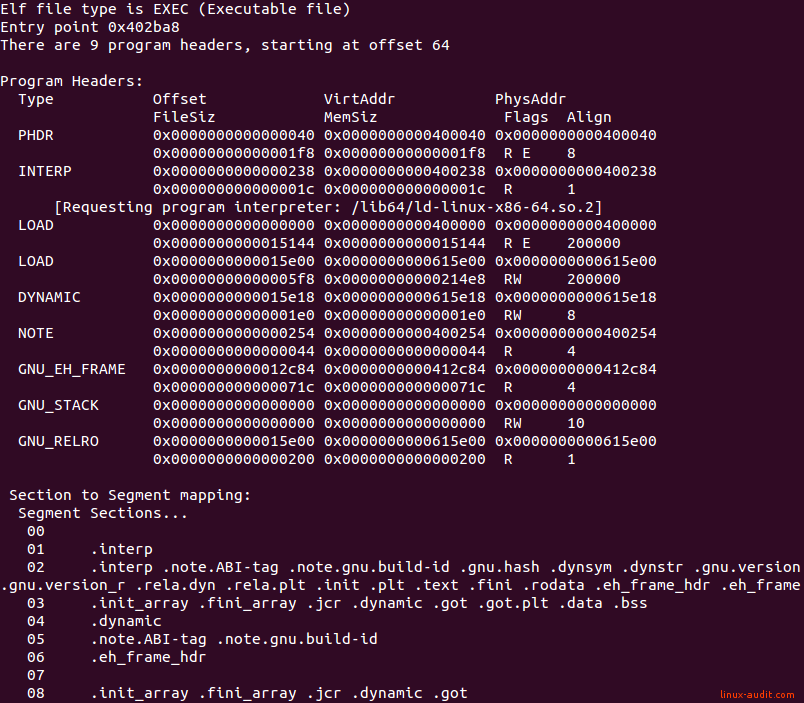
\includegraphics[scale=0.5]{images/elf-program-headers-segments.png}
        \caption{Programm Header einer Elf binary \cite{program_headers_of_Elf_binary}}
    \end{center}
\end{figure}

\subsubsection{GNU\_EH\_FRAME}
Dies ist eine sorted queue, die vom GNU C-Compiler (gcc) verwendet wird. Es speichert Ausnahmebehandlungsroutinen. Wenn also etwas schief geht, kann es diesen Bereich verwenden, um richtig damit umzugehen.

\subsubsection{GNU\_STACK}
Dieser Header wird zum Speichern von stack-Informationen verwendet. Der stack ist ein Puffer oder eine Arbeitsstelle, an der Elemente wie lokale Variablen gespeichert werden. Dies geschieht bei LIFO (Last In, First Out). Beim Starten einer Prozessfunktion wird ein Baustein reserviert. Wenn die Funktion beendet ist, wird sie wieder als frei markiert. Der interessante Teil ist nun, dass ein Stack nicht ausführbar sein sollte, da dies zu Sicherheitslücken führen kann. Durch Manipulation des Speichers könnte man auf diesen ausführbaren stack verweisen und beabsichtigte Anweisungen ausführen.

Wenn das Segment GNU\_STACK nicht verfügbar ist, wird normalerweise ein executable stack verwendet.
Die Tools scanelf und execstack sind zwei Beispiele, um die stack-Details anzuzeigen.

\begin{figure}[H]
    \begin{center}
        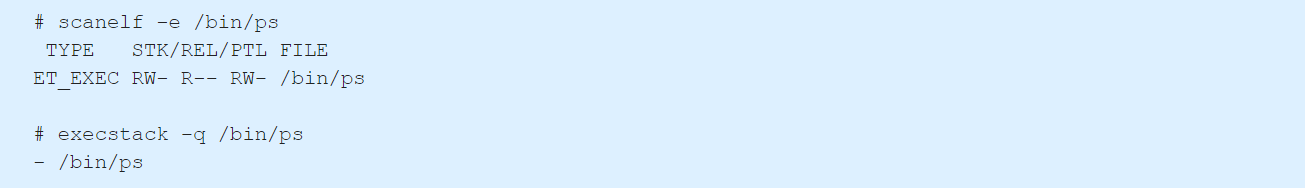
\includegraphics[scale=1]{images/example_gnustack.png}
        \caption{Beispiel GNU\_STACK \cite{example_gnustack}}
    \end{center}
\end{figure}